% Results. The earlier combined Results and Discussion draft remains available
% in results_discussion_draft.tex for comparison.

The three monitoring conditions differed in the availability of new MLCW information. Finalized monthly records became available after a temporary delay in one condition. The reduced-frequency condition provided one cumulative measurement every 6 or 12 months, whereas the final condition provided no subsequent MLCW measurement. The following subsections report how monthly and cumulative estimation errors changed across these conditions.

\subsection{Monthly estimation during delayed MLCW data delivery}
\label{subsec:results_delayed_delivery}

During delayed MLCW data delivery, estimated monthly increments followed the observed temporal patterns more closely in S1--S4 than in S5--S6. This comparison covered 23 complete six-month cycles from 05/2013 to 10/2024 and yielded 138 estimates for each depth section. After each cycle, the newly finalized monthly observations expanded the calibration record used for the next cycle (\Cref{fig:results_delayed_cycles}).

The monthly time series in \Cref{fig:results_delayed_monthly_estimates} show this contrast, and in \Cref{fig:results_delayed_scatter} the estimates for S1--S4 remained closer to the line of exact agreement than those for the two deepest sections.

\begin{figure}[htbp]
  \centering
  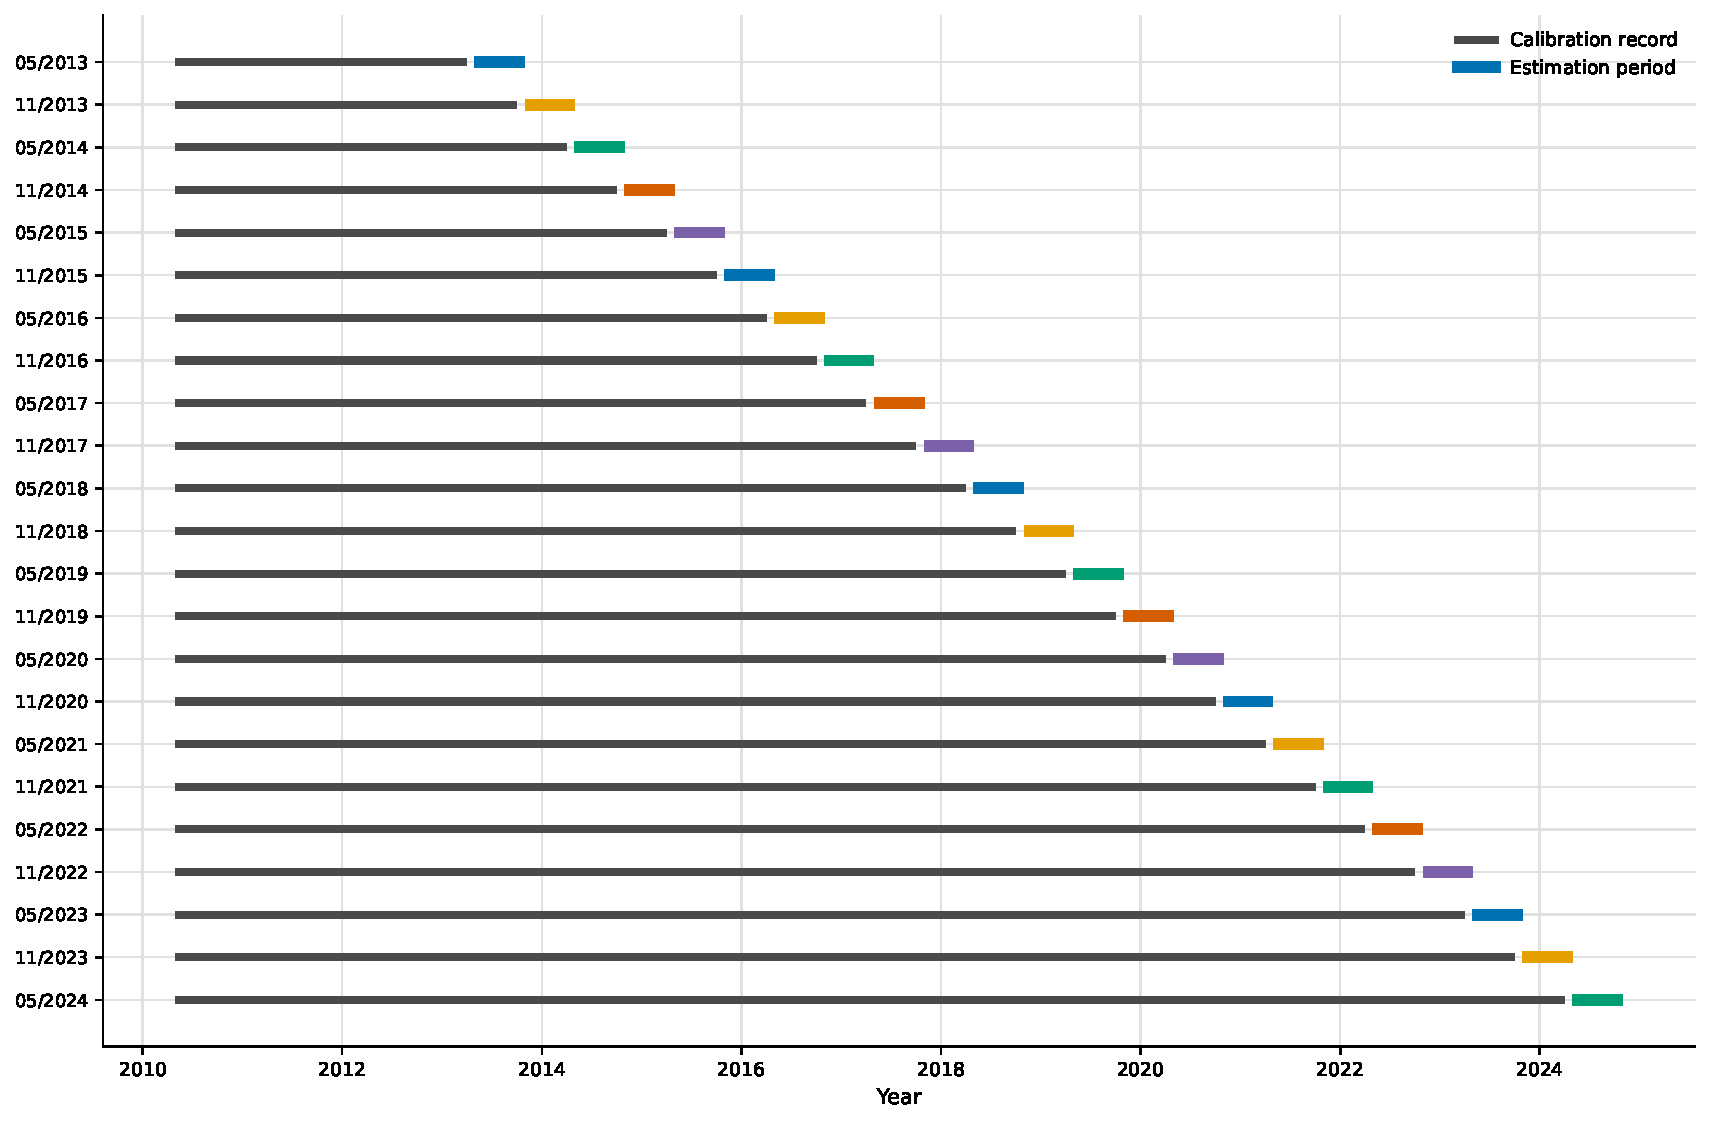
\includegraphics[width=0.98\textwidth]{figures/fig_results_delayed_cycle_timeline.pdf}
  \caption[Calibration and estimation periods during delayed MLCW data delivery.]{Successive calibration and estimation periods used to evaluate monthly deformation increments while finalized MLCW records were unavailable. The five colors repeat to distinguish adjacent estimation periods and do not represent different experimental conditions.}
  \label{fig:results_delayed_cycles}
\end{figure}

\begin{figure}[tp]
  \centering
  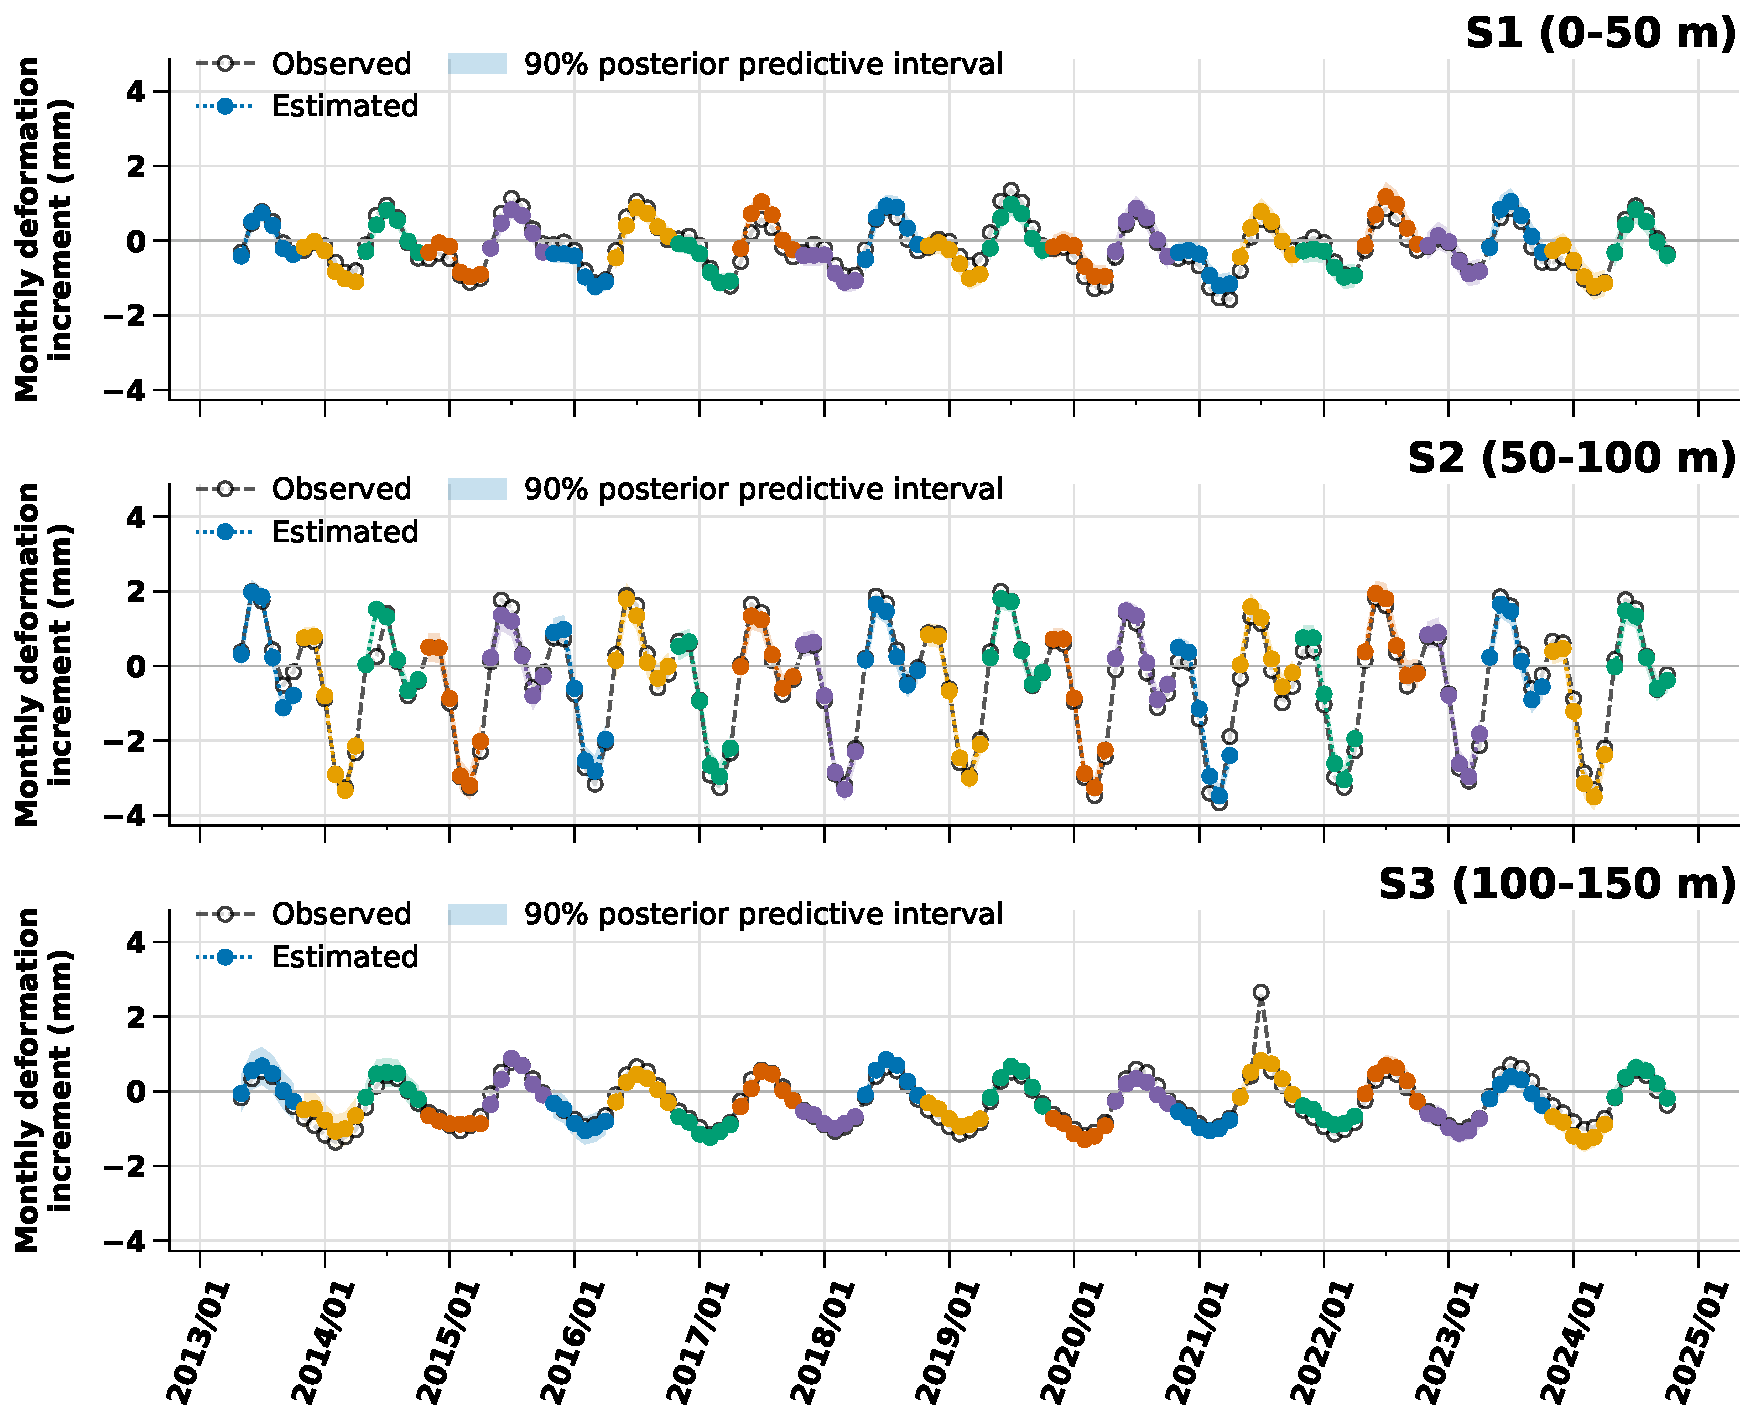
\includegraphics[width=0.98\textwidth]{figures/fig_results_delayed_monthly_estimates_s1_s3.pdf}
  \caption[Observed and estimated monthly deformation increments by depth section.]{Observed and estimated monthly deformation increments for S1--S3. The black lines show observations, colored dotted lines show estimates, and shaded bands show the 90\% Bayesian posterior predictive intervals, using the same repeating five-color scheme as \Cref{fig:results_delayed_cycles}.}
  \label{fig:results_delayed_monthly_estimates}
\end{figure}

\begin{figure}[tp]
  \ContinuedFloat
  \centering
  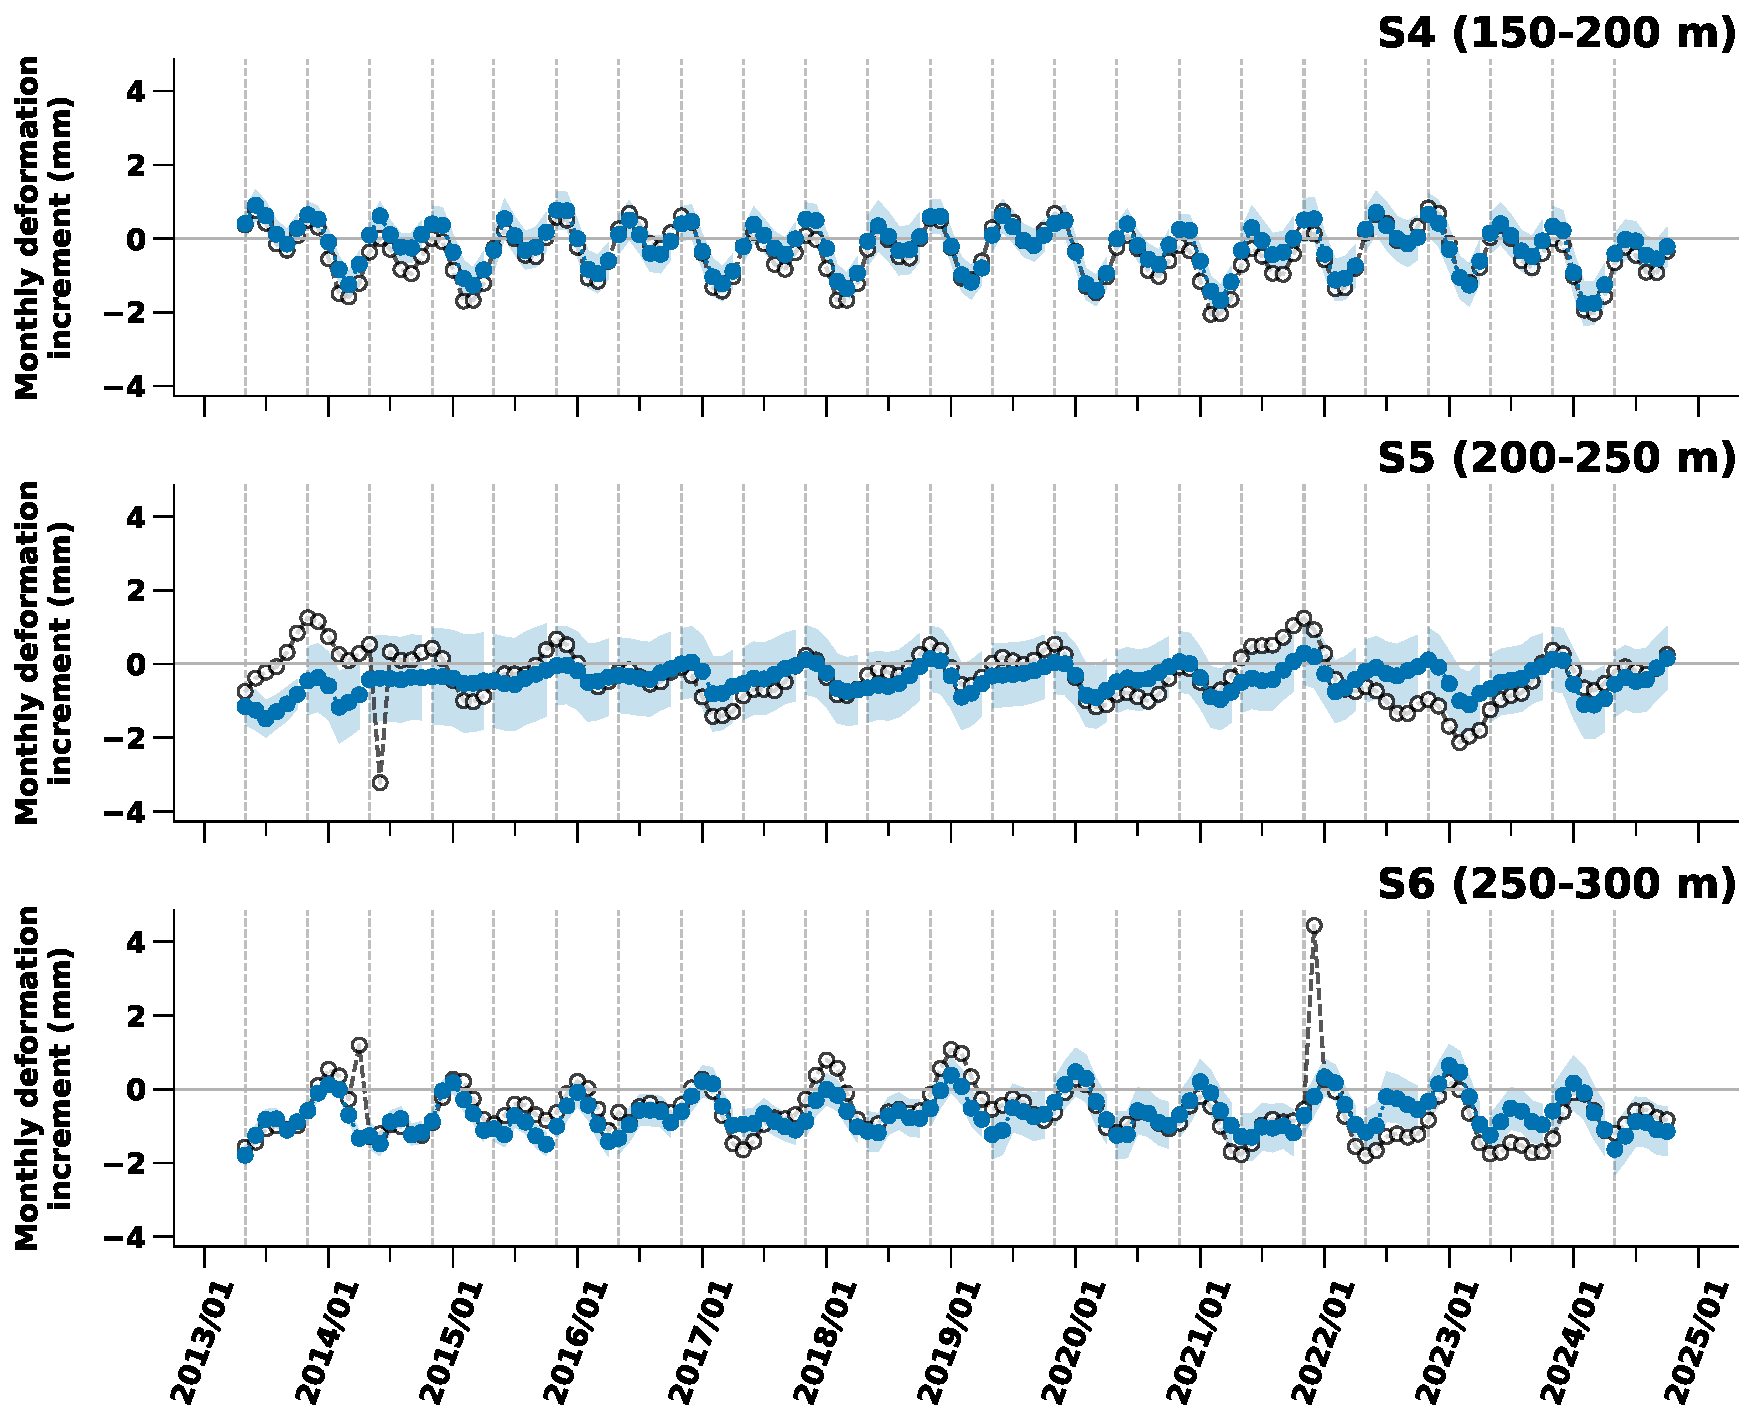
\includegraphics[width=0.98\textwidth]{figures/fig_results_delayed_monthly_estimates_s4_s6.pdf}
  \caption[]{Observed and estimated monthly deformation increments for S4--S6.}
\end{figure}

\begin{figure}[tp]
  \centering
  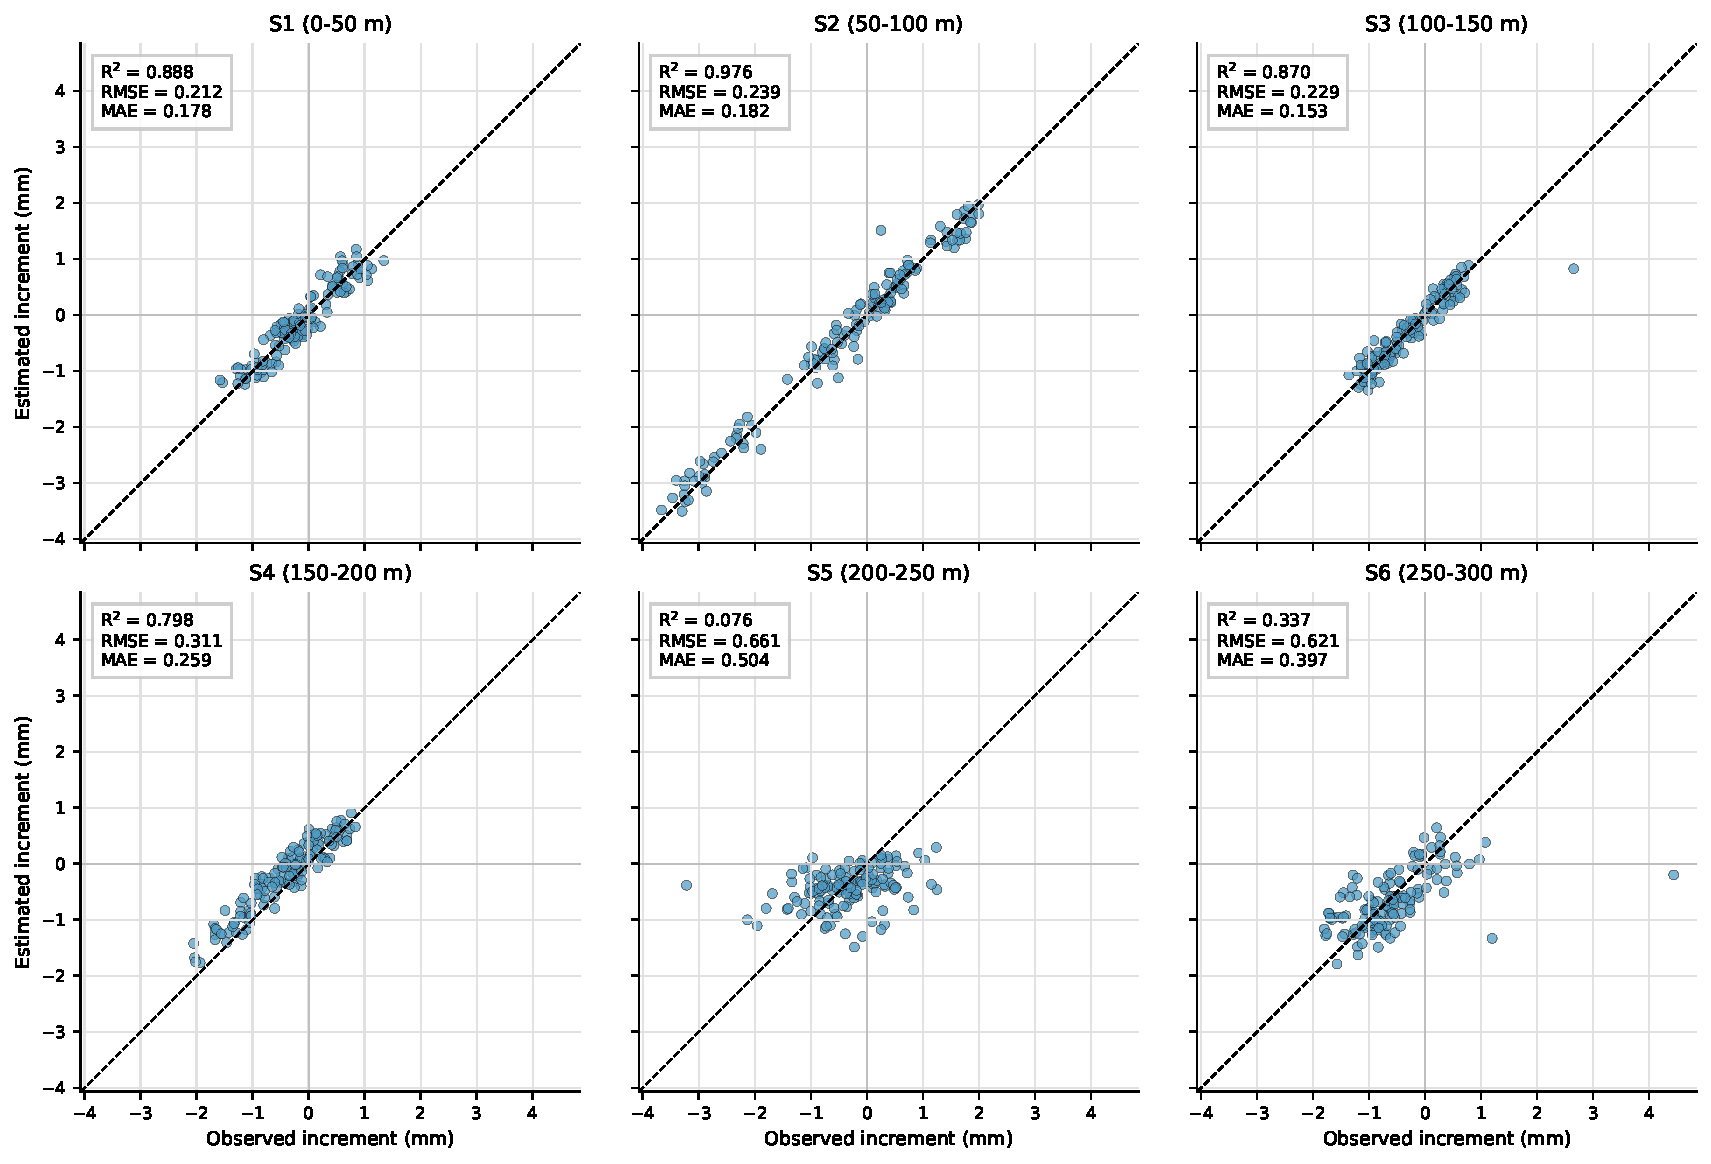
\includegraphics[width=0.98\textwidth]{figures/fig_results_delayed_prediction_vs_observed.pdf}
  \caption[Estimated versus observed monthly deformation increments.]{Estimated versus observed monthly deformation increments for the six depth sections. The dashed line represents exact agreement. RMSE and MAE are reported in mm/month.}
  \label{fig:results_delayed_scatter}
\end{figure}

\FloatBarrier

The depth contrast visible in the time series and scatter plots was also present in the error statistics (\Cref{tab:delayed_performance_interval}). Across the six depth sections, RMSE ranged from 0.21 to 0.66~mm/month and MAE ranged from 0.15 to 0.50~mm/month. Errors were smaller in S1--S4 than in S5 and S6, with S5 showing the largest RMSE and MAE.

The 90\% Bayesian posterior predictive intervals contained between 65.9\% and 88.4\% of the observations across the six sections, below the nominal 90\% level in every section, indicating the intervals were narrower than required. Possible sources of this gap are considered in \Cref{subsec:discussion_limitations}. Point-estimate error was worst in S5 and S6. Coverage, at 81.2\% in S5 and 65.9\% in S6, was not worst in both of those same sections. It reached its lowest value in S6, while S1 (74.6\%) and S3 (73.9\%) also fell below S5. Reliability therefore did not follow the same depth pattern as point-estimate error.

% Source: diag_28_sec4_meansd_tables.py (sec4_1 window, station=TUKU, datetime<=2024-10-01;
% reproduces performance_by_section.csv / interval_coverage_by_section.csv exactly)
\begin{table}[htbp]
  \centering
  \small
  \renewcommand{\arraystretch}{1.15}
  \caption[Performance and posterior predictive interval statistics during delayed MLCW delivery.]{Point-estimate errors, model fit, and 90\% posterior predictive interval statistics for monthly deformation estimates, one row per depth section ($n=138$ estimates each). Metrics defined in \Cref{tab:evaluation_metrics}.}
  \label{tab:delayed_performance_interval}
  \begin{tabular}{l|r|r|r|r|r}
    \toprule
    \multicolumn{1}{c|}{\textbf{Section}} & \multicolumn{1}{c|}{\textbf{$R^2$}} & \multicolumn{1}{c|}{\textbf{RMSE}} & \multicolumn{1}{c|}{\textbf{MAE}} & \multicolumn{1}{c|}{\textbf{Coverage (\%)}} & \multicolumn{1}{c}{\textbf{Width}} \\
    \midrule
    S1 & 0.89 & 0.21 & 0.18 & 74.6 & 0.54 \\
    S2 & 0.98 & 0.24 & 0.18 & 88.4 & 0.64 \\
    S3 & 0.87 & 0.23 & 0.15 & 73.9 & 0.44 \\
    S4 & 0.80 & 0.31 & 0.26 & 84.8 & 0.98 \\
    S5 & 0.08 & 0.66 & 0.50 & 81.2 & 1.85 \\
    S6 & 0.34 & 0.62 & 0.40 & 65.9 & 0.97 \\
    \bottomrule
  \end{tabular}
\end{table}

Monthly estimation errors did not increase steadily with time since the preceding MLCW update (\Cref{tab:delayed_performance_by_month}). Mean MAE ranged from 0.25 to 0.34~mm/month across the six month positions, with the highest value at position 2 rather than position 6. $R^2$ varied more widely among positions than either error metric, from a mean of 0.34 at position 1 to a mean of 0.61 at position 4, with the standard deviation across sections at every position ($0.2$--$0.5$) reflecting the same S1--S4 versus S5--S6 depth contrast already visible in \Cref{tab:delayed_performance_interval}.

% Source: diag_28_sec4_meansd_tables.py (sec4_1_by_month.csv; per-section-then-mean+-SD, n=6 sections per cell)
\begin{table}[htbp]
  \centering
  \small
  \renewcommand{\arraystretch}{1.15}
  \caption[Performance by month position within each estimation cycle.]{Performance by months since the last cumulative MLCW update (month 1--6 of each six-month cycle, not calendar months). Mean $\pm$ SD, $n=6$ sections; metrics per \Cref{tab:evaluation_metrics}.}
  \label{tab:delayed_performance_by_month}
  \begin{tabular}{l|r|r|r|r|r}
    \toprule
    \multicolumn{1}{c|}{\textbf{Months since retrain}} & \multicolumn{1}{c|}{\textbf{$R^2$}} & \multicolumn{1}{c|}{\textbf{MAE}} & \multicolumn{1}{c|}{\textbf{RMSE}} & \multicolumn{1}{c|}{\textbf{Coverage (\%)}} & \multicolumn{1}{c}{\textbf{Width}} \\
    \midrule
    1 & $0.34\pm0.2$ & $0.25\pm0.1$ & $0.31\pm0.2$ & $80.4\pm7.7$ & $0.91\pm0.5$ \\
    2 & $0.43\pm0.4$ & $0.34\pm0.2$ & $0.50\pm0.4$ & $73.2\pm14.1$ & $0.91\pm0.5$ \\
    3 & $0.57\pm0.5$ & $0.27\pm0.1$ & $0.36\pm0.2$ & $79.0\pm10.1$ & $0.91\pm0.5$ \\
    4 & $0.61\pm0.5$ & $0.28\pm0.1$ & $0.34\pm0.2$ & $74.6\pm8.4$ & $0.90\pm0.5$ \\
    5 & $0.58\pm0.5$ & $0.26\pm0.1$ & $0.32\pm0.2$ & $82.6\pm9.9$ & $0.90\pm0.5$ \\
    6 & $0.49\pm0.5$ & $0.28\pm0.2$ & $0.37\pm0.2$ & $79.0\pm11.8$ & $0.90\pm0.5$ \\
    \bottomrule
  \end{tabular}
\end{table}

\FloatBarrier

The fitted coefficients also varied among depth sections. To summarize these differences without reproducing all model coefficients, \Cref{tab:selected_coefficients} presents 14 variables whose 10th--90th percentile range remained entirely positive or negative in at least one section.

\begin{sidewaystable}[p]
  \centering
  \footnotesize
  \renewcommand{\arraystretch}{1.25}
  \setlength{\tabcolsep}{3.5pt}
  \caption[Selected standardized coefficients across depth sections.]{Selected standardized coefficients across the six depth sections. Each cell gives the median and the range from the 10th to the 90th percentile after combining coefficient results from 24 model updates with equal weight, including the update from the final, partially scored six-month cycle. Bold marks ranges that were entirely positive or negative; a dash means that the variable was not used for that section.}
  \label{tab:selected_coefficients}
  \begin{tabular}{@{}p{0.29\textheight}|*{5}{c|}c@{}}
    \toprule
    \textbf{Driving feature} & \textbf{S1} & \textbf{S2} & \textbf{S3} & \textbf{S4} & \textbf{S5} & \textbf{S6} \\
    \midrule
    \multicolumn{7}{@{}l}{\textit{Surface-displacement predictors}} \\
    Current surface-displacement increment & \makecell{$\mathbf{0.206}$\\$\mathbf{[0.140,\ 0.230]}$} & \makecell{$\mathbf{0.515}$\\$\mathbf{[0.437,\ 0.573]}$} & \makecell{$\mathbf{0.479}$\\$\mathbf{[0.069,\ 0.809]}$} & \makecell{$\mathbf{0.236}$\\$\mathbf{[0.189,\ 0.332]}$} & \makecell{$0.009$\\$[-0.065,\ 0.030]$} & \makecell{$\mathbf{0.183}$\\$\mathbf{[0.121,\ 0.230]}$} \\
    Change in surface-displacement increment & \makecell{$0.028$\\$[-0.011,\ 0.039]$} & \makecell{$\mathbf{0.325}$\\$\mathbf{[0.303,\ 0.377]}$} & \makecell{$\mathbf{0.340}$\\$\mathbf{[0.079,\ 0.458]}$} & \makecell{$\mathbf{0.192}$\\$\mathbf{[0.170,\ 0.229]}$} & \makecell{$\mathbf{0.045}$\\$\mathbf{[0.010,\ 0.058]}$} & \makecell{$\mathbf{-0.044}$\\$\mathbf{[-0.064,\ -0.021]}$} \\
    Surface-displacement increment, 1-month lag & \makecell{$\mathbf{0.181}$\\$\mathbf{[0.151,\ 0.197]}$} & \makecell{$\mathbf{0.210}$\\$\mathbf{[0.141,\ 0.233]}$} & \makecell{$\mathbf{0.167}$\\$\mathbf{[0.006,\ 0.404]}$} & \makecell{$0.058$\\$[0.034,\ 0.124]$} & \makecell{$\mathbf{-0.027}$\\$\mathbf{[-0.112,\ -0.012]}$} & \makecell{$\mathbf{0.226}$\\$\mathbf{[0.169,\ 0.259]}$} \\
    Surface-displacement increment, 3-month lag & \makecell{$\mathbf{0.026}$\\$\mathbf{[0.001,\ 0.045]}$} & \makecell{$\mathbf{-0.297}$\\$\mathbf{[-0.378,\ -0.252]}$} & \makecell{$\mathbf{-0.769}$\\$\mathbf{[-1.308,\ -0.221]}$} & \makecell{$0.016$\\$[-0.027,\ 0.133]$} & \makecell{$\mathbf{-0.014}$\\$\mathbf{[-0.140,\ -0.001]}$} & \makecell{$\mathbf{0.160}$\\$\mathbf{[0.074,\ 0.203]}$} \\
    \midrule
    \multicolumn{7}{@{}l}{\textit{Hydraulic-head predictors}} \\
    Magnitude of hydraulic-head change & \makecell{$\mathbf{-0.046}$\\$\mathbf{[-0.064,\ -0.028]}$} & \makecell{$\mathbf{-0.037}$\\$\mathbf{[-0.046,\ -0.030]}$} & \makecell{$-0.003$\\$[-0.007,\ 0.007]$} & \makecell{$\mathbf{0.028}$\\$\mathbf{[0.015,\ 0.040]}$} & \makecell{$-0.025$\\$[-0.031,\ 0.012]$} & \makecell{$0.006$\\$[-0.031,\ 0.037]$} \\
    Hydraulic-head change, 12-month lag & \makecell{$\mathbf{0.039}$\\$\mathbf{[0.018,\ 0.061]}$} & \makecell{$\mathbf{0.052}$\\$\mathbf{[0.041,\ 0.113]}$} & \makecell{$0.015$\\$[-0.009,\ 0.032]$} & \makecell{$\mathbf{0.016}$\\$\mathbf{[0.001,\ 0.027]}$} & \makecell{$-0.003$\\$[-0.091,\ 0.010]$} & \makecell{$0.014$\\$[-0.030,\ 0.046]$} \\
    Hydraulic-head change, 24-month lag & \makecell{$\mathbf{0.032}$\\$\mathbf{[0.019,\ 0.045]}$} & \makecell{$0.008$\\$[-0.017,\ 0.032]$} & \makecell{$\mathbf{-0.026}$\\$\mathbf{[-0.040,\ -0.004]}$} & \makecell{$\mathbf{-0.035}$\\$\mathbf{[-0.067,\ -0.016]}$} & \makecell{$\mathbf{0.033}$\\$\mathbf{[0.014,\ 0.070]}$} & \makecell{$\mathbf{0.077}$\\$\mathbf{[0.026,\ 0.114]}$} \\
    S1 hydraulic-head change, 6-month trailing mean & -- & \makecell{$\mathbf{0.183}$\\$\mathbf{[0.122,\ 0.269]}$} & \makecell{$\mathbf{0.101}$\\$\mathbf{[0.010,\ 0.223]}$} & \makecell{$\mathbf{0.125}$\\$\mathbf{[0.105,\ 0.151]}$} & \makecell{$\mathbf{0.025}$\\$\mathbf{[0.014,\ 0.078]}$} & \makecell{$-0.056$\\$[-0.113,\ 0.111]$} \\
    S6 hydraulic-head change, 6-month trailing mean & \makecell{$\mathbf{-0.091}$\\$\mathbf{[-0.204,\ -0.050]}$} & \makecell{$\mathbf{0.074}$\\$\mathbf{[0.020,\ 0.150]}$} & \makecell{$0.015$\\$[-0.027,\ 0.063]$} & \makecell{$\mathbf{0.067}$\\$\mathbf{[0.038,\ 0.082]}$} & \makecell{$\mathbf{0.023}$\\$\mathbf{[0.011,\ 0.064]}$} & -- \\
    \midrule
    \multicolumn{7}{@{}l}{\textit{Seasonal predictors}} \\
    Dry-season indicator & \makecell{$\mathbf{-0.139}$\\$\mathbf{[-0.154,\ -0.130]}$} & \makecell{$\mathbf{-0.214}$\\$\mathbf{[-0.256,\ -0.184]}$} & \makecell{$\mathbf{-0.083}$\\$\mathbf{[-0.161,\ -0.045]}$} & \makecell{$\mathbf{-0.059}$\\$\mathbf{[-0.079,\ -0.046]}$} & \makecell{$\mathbf{-0.014}$\\$\mathbf{[-0.042,\ -0.000]}$} & \makecell{$\mathbf{0.111}$\\$\mathbf{[0.047,\ 0.165]}$} \\
    Annual sine component & \makecell{$\mathbf{-0.212}$\\$\mathbf{[-0.257,\ -0.143]}$} & \makecell{$\mathbf{-0.542}$\\$\mathbf{[-0.591,\ -0.413]}$} & \makecell{$\mathbf{-0.108}$\\$\mathbf{[-0.263,\ -0.018]}$} & \makecell{$\mathbf{-0.054}$\\$\mathbf{[-0.078,\ -0.020]}$} & \makecell{$\mathbf{-0.072}$\\$\mathbf{[-0.133,\ -0.032]}$} & \makecell{$\mathbf{0.140}$\\$\mathbf{[0.085,\ 0.167]}$} \\
    Annual cosine component & \makecell{$-0.030$\\$[-0.080,\ 0.012]$} & \makecell{$-0.034$\\$[-0.059,\ 0.007]$} & \makecell{$-0.011$\\$[-0.231,\ 0.253]$} & \makecell{$-0.028$\\$[-0.065,\ 0.024]$} & \makecell{$\mathbf{0.053}$\\$\mathbf{[0.021,\ 0.081]}$} & \makecell{$\mathbf{0.312}$\\$\mathbf{[0.249,\ 0.379]}$} \\
    Semiannual sine component & \makecell{$\mathbf{0.033}$\\$\mathbf{[0.029,\ 0.048]}$} & \makecell{$\mathbf{-0.150}$\\$\mathbf{[-0.179,\ -0.118]}$} & \makecell{$-0.171$\\$[-0.540,\ 0.003]$} & \makecell{$\mathbf{-0.134}$\\$\mathbf{[-0.166,\ -0.103]}$} & \makecell{$\mathbf{-0.036}$\\$\mathbf{[-0.048,\ -0.012]}$} & \makecell{$\mathbf{0.072}$\\$\mathbf{[0.050,\ 0.104]}$} \\
    Semiannual cosine component & \makecell{$\mathbf{0.046}$\\$\mathbf{[0.018,\ 0.071]}$} & \makecell{$0.113$\\$[-0.044,\ 0.141]$} & \makecell{$\mathbf{-1.257}$\\$\mathbf{[-2.167,\ -0.197]}$} & \makecell{$\mathbf{0.087}$\\$\mathbf{[0.054,\ 0.095]}$} & \makecell{$\mathbf{0.048}$\\$\mathbf{[0.018,\ 0.061]}$} & \makecell{$-0.011$\\$[-0.059,\ 0.012]$} \\
    \bottomrule
  \end{tabular}
\end{sidewaystable}

\FloatBarrier

Surface-displacement terms showed the clearest repeated directional patterns across the depth sections. The current increment had a positive coefficient range in S1--S4 and S6, whereas the hydraulic-head terms showed fewer common patterns among sections. Seasonal coefficients also varied with depth, with the dry-season indicator and annual sine component having opposite directions in S6 and the five shallower sections. These results describe fitted associations and are interpreted separately in \Cref{sec:discussion}.

Each monthly estimate used hydraulic-head and cGNSS observations available through the corresponding month, including the specified lagged changes, so the evaluation did not represent forecasts made before those observations became available. Point-estimate errors were larger in S5 and S6 than in S1--S4. Posterior predictive coverage did not follow this same depth pattern. It fell below the nominal 90\% level in every section and reached its lowest value in S6.

\FloatBarrier

\subsection{Estimation under reduced MLCW measurement frequency}
\label{subsec:results_reduced_frequency}

Less frequent MLCW field measurements changed the error at the next cumulative observation more clearly than the error in individual monthly estimates. Monthly hydraulic-head and cGNSS observations remained available between MLCW measurements, and the hidden monthly MLCW observations were used only for retrospective evaluation. The 3-, 5-, and 8-year initial records were evaluated over the same 72 months from 05/2018 to 04/2024, giving 72 endpoint comparisons under the 6-month schedule and 36 under the 12-month schedule.

The 3-year initial record provided the visual example for both measurement intervals (\Cref{fig:results_reduced_frequency_3yr}).

\begin{figure}[tp]
  \centering
  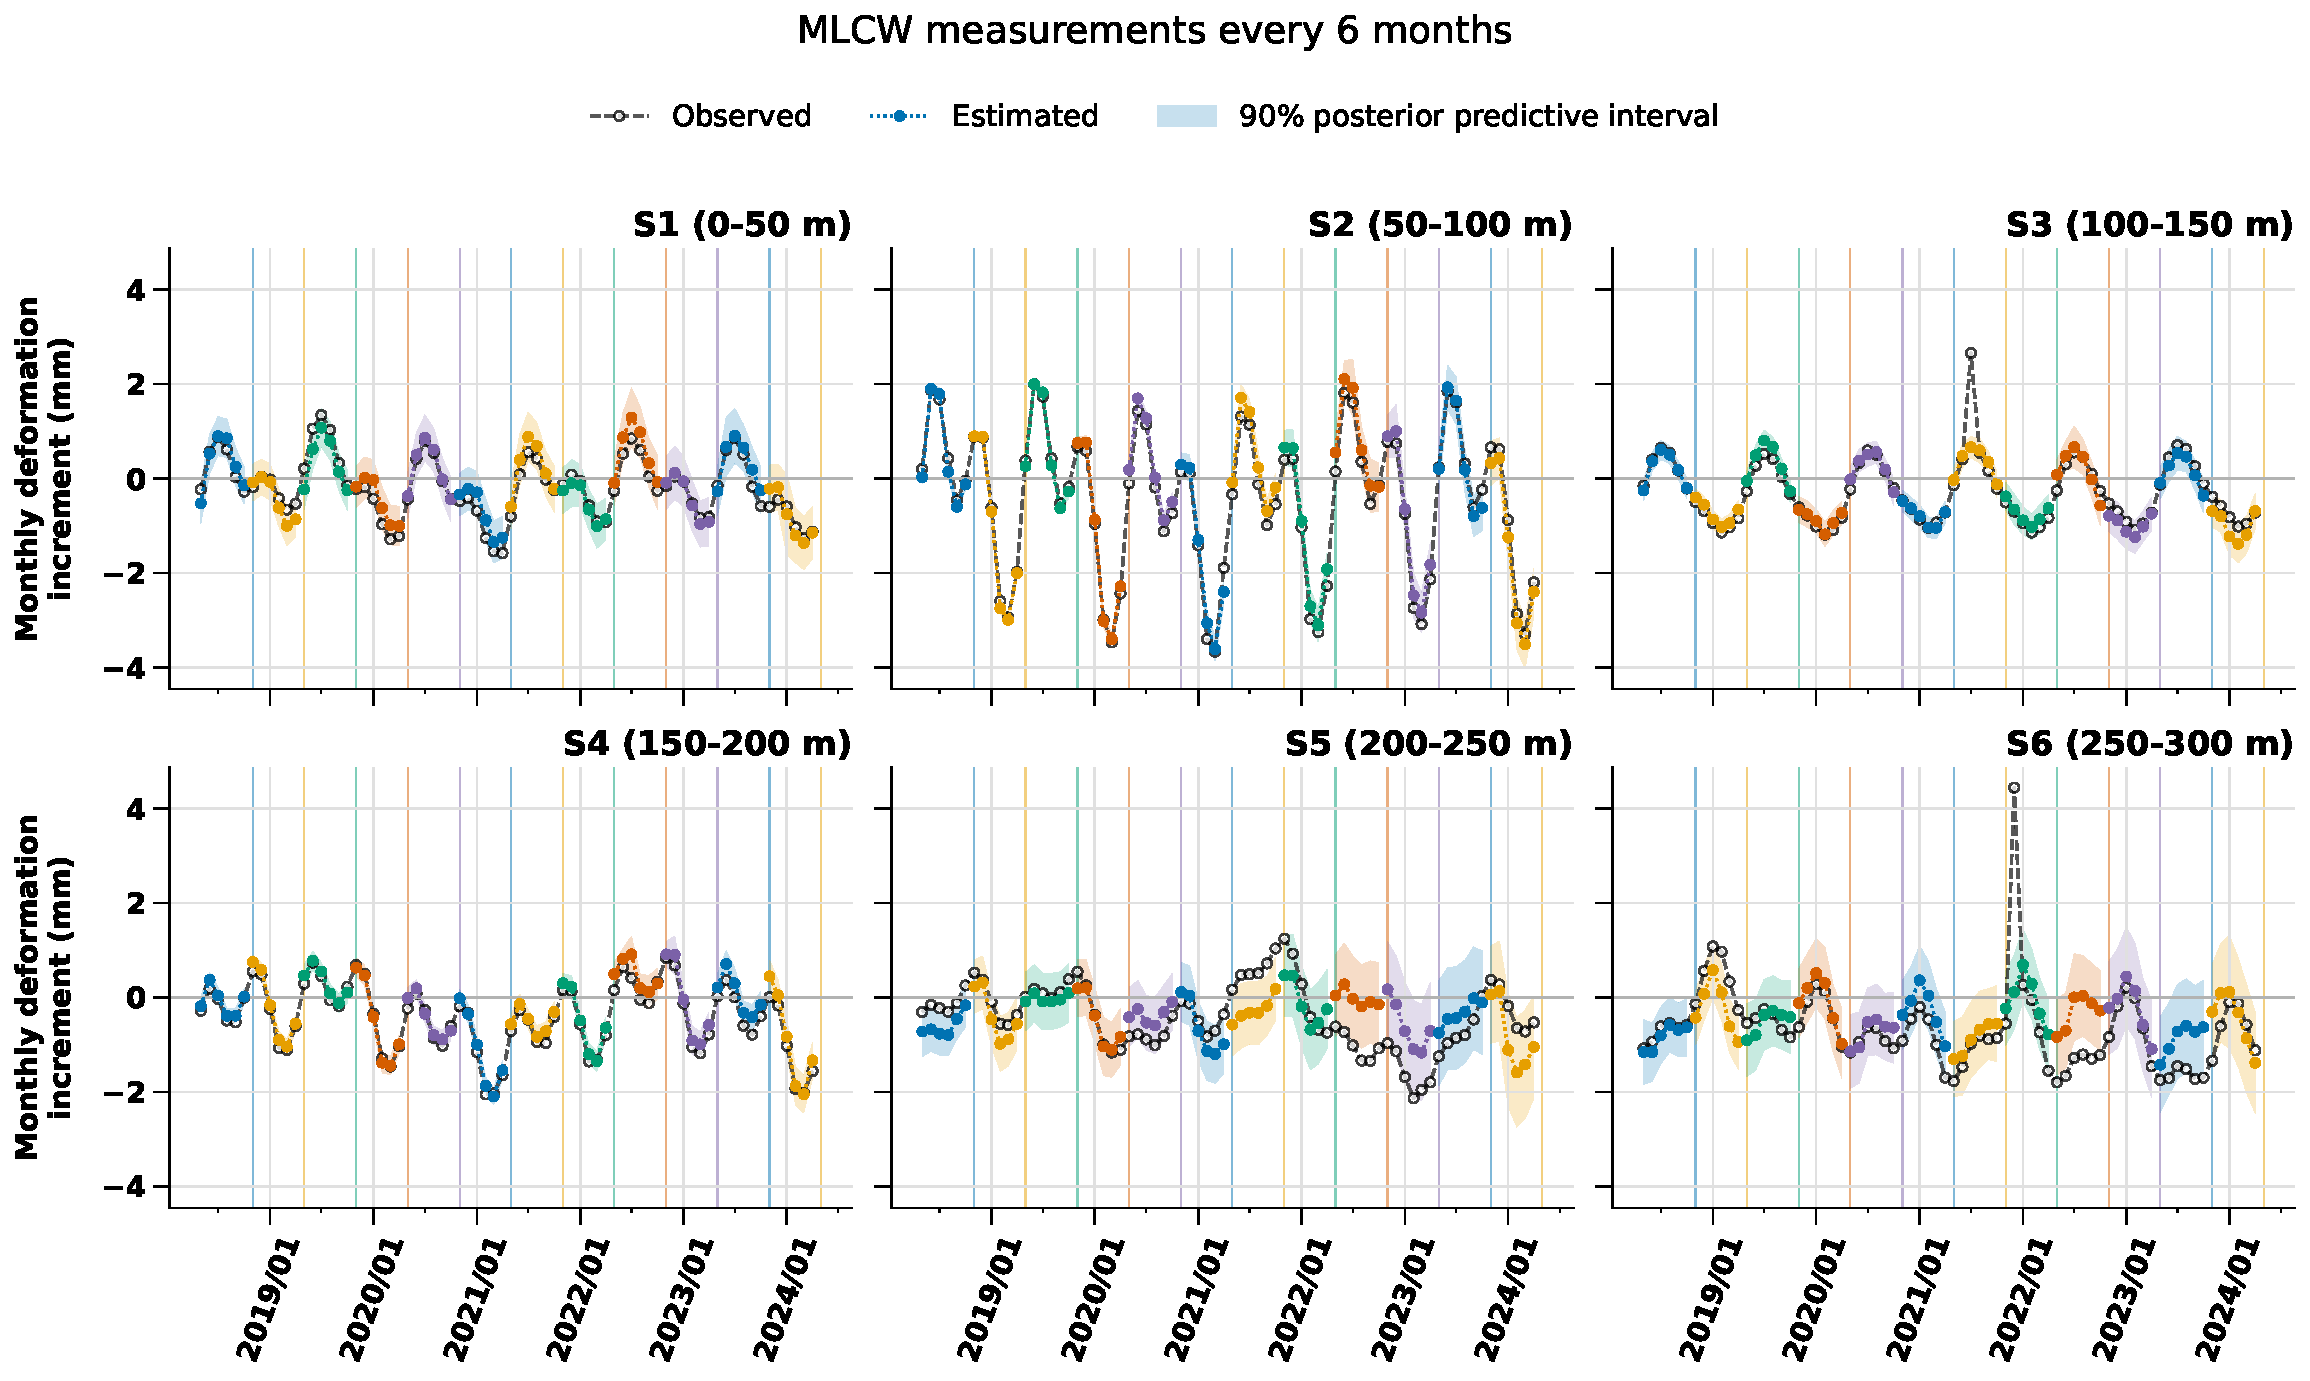
\includegraphics[width=0.98\textwidth]{figures/fig_results_reduced_frequency_3yr_panel_a.pdf}
  \caption[Observed and estimated monthly deformation increments under reduced MLCW measurement frequency.]{Observed and estimated monthly deformation increments for the 3-year initial record, all six depth sections, evaluated over the shared 05/2018--04/2024 period. (a) 6-month measurement schedule. Vertical lines mark the months when a new cumulative MLCW field measurement became available for the next update.}
  \label{fig:results_reduced_frequency_3yr}
\end{figure}

\begin{figure}[tp]
  \ContinuedFloat
  \centering
  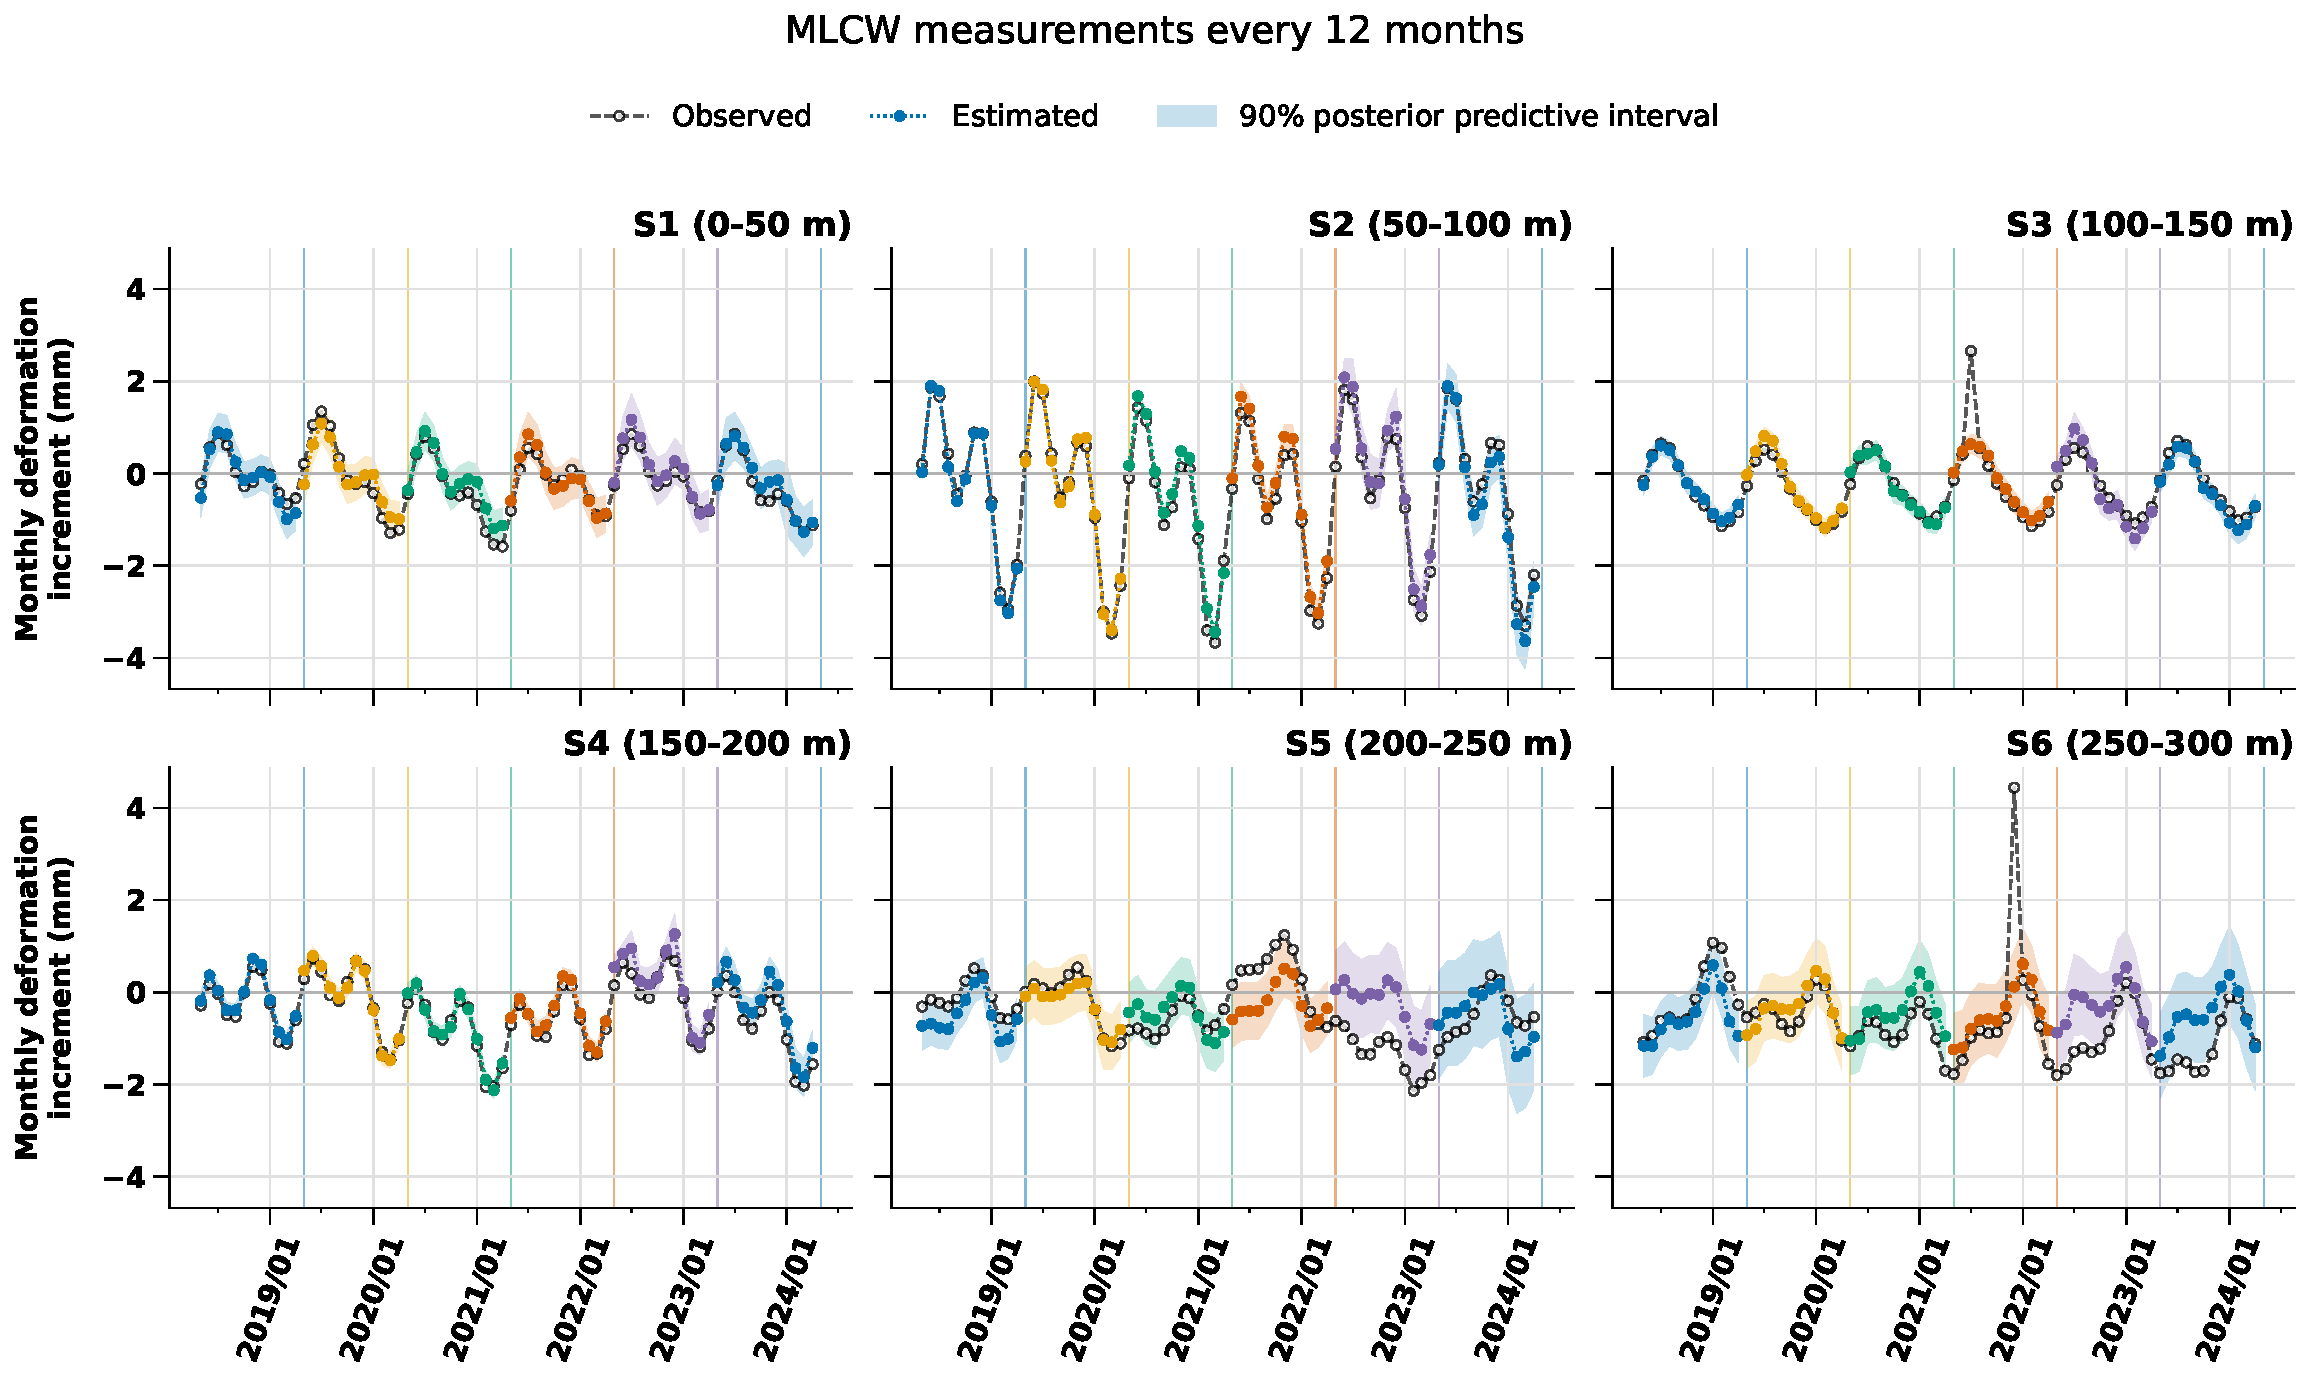
\includegraphics[width=0.98\textwidth]{figures/fig_results_reduced_frequency_3yr_panel_b.pdf}
  \caption[]{(b) 12-month measurement schedule.}
\end{figure}

\FloatBarrier

% Source: diag_28_sec4_meansd_tables.py (sec4_2_meansd.csv; per-section-then-mean+-SD, n=6 sections per row)
\begin{table}[htbp]
  \centering
  \footnotesize
  \setlength{\tabcolsep}{3pt}
  \renewcommand{\arraystretch}{1.2}
  \caption[Monthly errors under reduced MLCW measurement frequency.]{Monthly errors at Tuku, evaluated over the identical 72-month period (05/2018--04/2024) in every scenario. Mean $\pm$ SD, $n=6$ sections; metrics per \Cref{tab:evaluation_metrics}. Full per-section values: \Cref{supp-tab:supp_reduced_frequency_monthly_full}.}
  \label{tab:results_reduced_frequency}
  \begin{tabular}{c|c|r|r|r|r|r}
    \toprule
    \multicolumn{1}{c|}{\shortstack{\textbf{Sampling}\\\textbf{interval}\\\textbf{(months)}}} & \multicolumn{1}{c|}{\shortstack{\textbf{Initial}\\\textbf{record}\\\textbf{(years)}}} & \multicolumn{1}{c|}{\textbf{$R^2$}} & \multicolumn{1}{c|}{\textbf{MAE}} & \multicolumn{1}{c|}{\textbf{RMSE}} & \multicolumn{1}{c|}{\textbf{Coverage (\%)}} & \multicolumn{1}{c}{\textbf{Width}} \\
    \midrule
    6  & 3 & $0.70\pm0.3$ & $0.28\pm0.2$ & $0.37\pm0.2$ & $82.9\pm9.6$ & $0.94\pm0.5$ \\
    6  & 5 & $0.68\pm0.4$ & $0.27\pm0.2$ & $0.38\pm0.3$ & $89.4\pm9.5$ & $1.11\pm0.8$ \\
    6  & 8 & $0.67\pm0.3$ & $0.30\pm0.1$ & $0.40\pm0.2$ & $87.3\pm9.0$ & $1.35\pm0.8$ \\
    \midrule
    12 & 3 & $0.69\pm0.3$ & $0.29\pm0.2$ & $0.39\pm0.2$ & $77.8\pm9.5$ & $0.87\pm0.5$ \\
    12 & 5 & $0.68\pm0.4$ & $0.27\pm0.2$ & $0.38\pm0.2$ & $86.6\pm12.7$ & $1.07\pm0.7$ \\
    12 & 8 & $0.66\pm0.3$ & $0.31\pm0.1$ & $0.41\pm0.2$ & $81.9\pm12.0$ & $1.32\pm0.9$ \\
    \bottomrule
  \end{tabular}
\end{table}

Mean monthly MAE across the six depth sections remained between 0.27 and 0.31~mm/month across the six scenarios (\Cref{tab:results_reduced_frequency}). Mean $R^2$ ranged from 0.66 to 0.70 and did not differ consistently between the 6-month and 12-month schedules. In every scenario the standard deviation across sections was large relative to the mean --- for $R^2$, the standard deviation exceeded 0.3 in all six scenarios --- reflecting the same S1--S4 versus S5--S6 depth contrast already documented in \Cref{subsec:results_delayed_delivery}; full per-section values are given in \Cref{supp-tab:supp_reduced_frequency_monthly_full}.

Extending the initial record from 3 to 8 years did not reduce mean monthly MAE consistently. The 5-year record produced the lowest mean monthly MAE under both schedules, whereas the 8-year record produced the highest. Mean coverage of the nominal 90\% intervals ranged from 77.8 to 89.4\%, remaining below the nominal level in all six scenarios on average. As in \Cref{subsec:results_delayed_delivery}, this shortfall reflects the discrepancy between the observed coverage and the nominal interval level rather than a difference in interval width; possible mechanisms are discussed in \Cref{subsec:discussion_limitations}.

\FloatBarrier

\subsection{Estimation without subsequent MLCW measurements}
\label{subsec:results_no_subsequent_mlcw}

Without subsequent MLCW measurements, monthly errors remained within a narrow range among the three initial-record lengths. Each model was calibrated once and evaluated over the same 80 months from 05/2018 to 12/2024 while monthly hydraulic-head and cGNSS observations remained available. Averaged across the six depth sections, mean monthly MAE ranged from 0.26 to 0.29~mm/month and mean RMSE ranged from 0.36 to 0.40~mm/month across the three initial-record lengths (\Cref{tab:results_no_subsequent_mlcw_interval}).

Cumulative errors varied among depth sections and, by month 80, ended at different values (\Cref{fig:results_no_subsequent_mlcw_cumulative_error}). At the end of the 80-month evaluation period, S4 had the largest absolute cumulative error under all three initial-record lengths (\Cref{tab:results_no_subsequent_mlcw_h80}). The 8-year initial record reduced this error in S4--S6. It did not produce the smallest value in every section. The 5-year record performed better than the 8-year record in S1 and S2.

\begin{figure}[htbp]
  \centering
  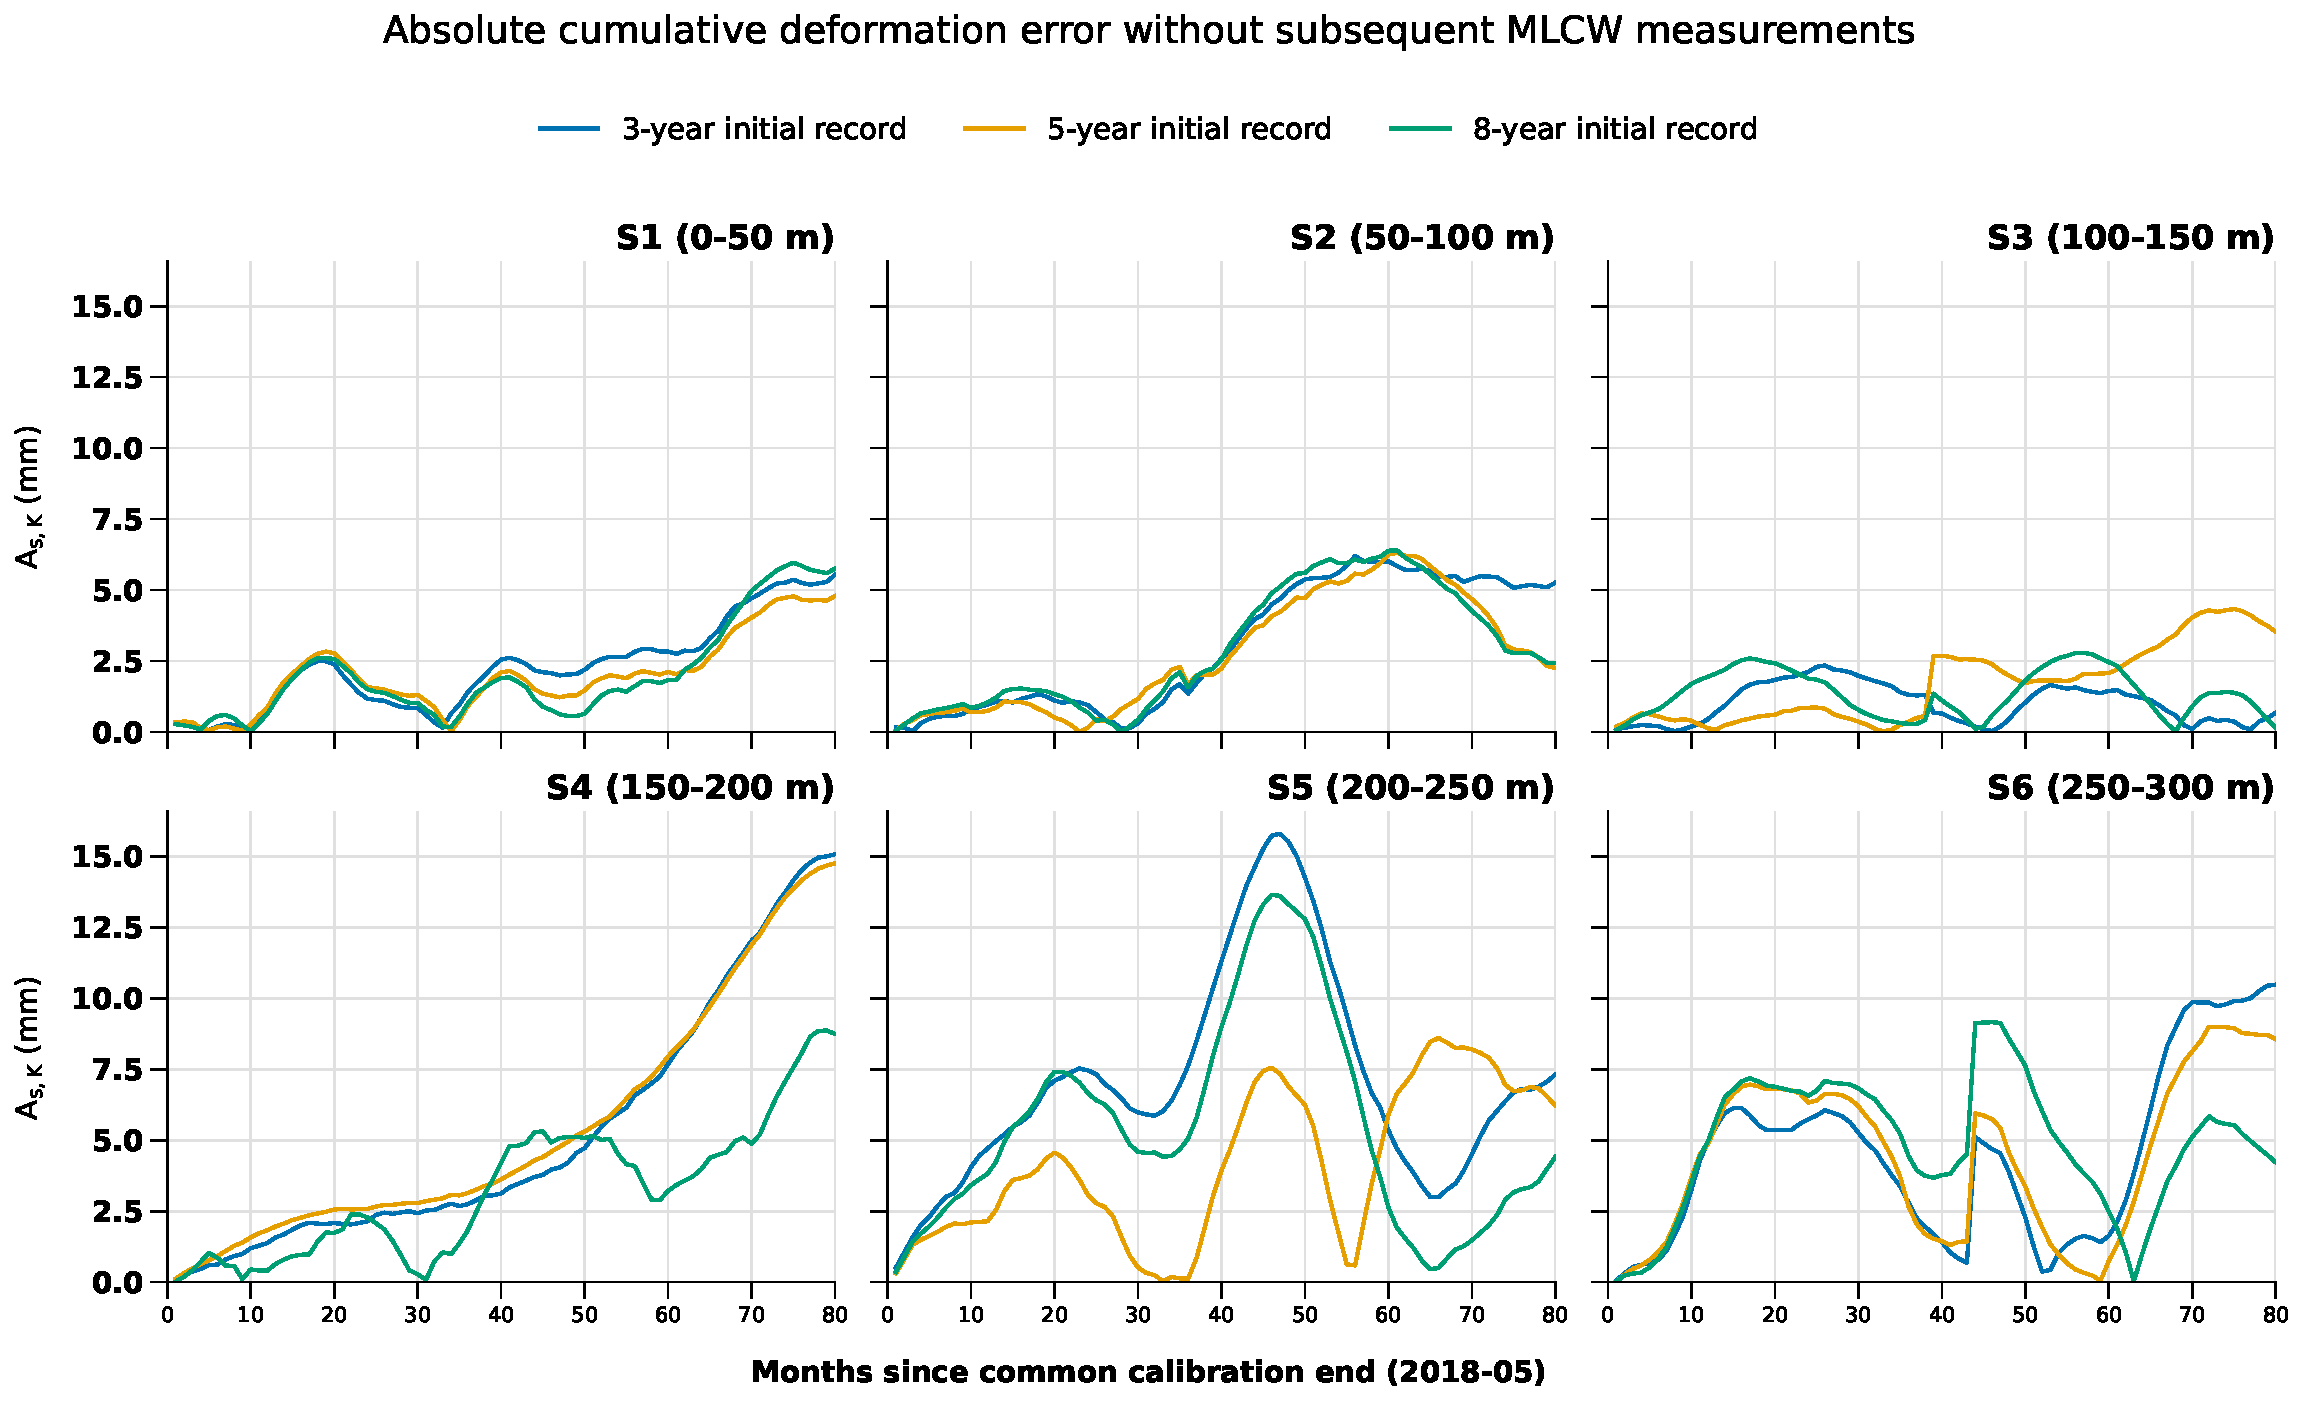
\includegraphics[width=0.98\textwidth]{figures/fig_results_no_subsequent_mlcw_cumulative_error.pdf}
  \caption[Absolute cumulative deformation error without subsequent MLCW measurements.]{Absolute cumulative deformation error $A_{s,K}=|E_{s,K}|$ for each depth section against months since the shared calibration endpoint (05/2018), shown separately for the 3-, 5-, and 8-year initial records, evaluated over the shared 80-month period.}
  \label{fig:results_no_subsequent_mlcw_cumulative_error}
\end{figure}

\begin{table}[htbp]
  \centering
  \small
  \renewcommand{\arraystretch}{1.15}
  \caption[Absolute cumulative deformation error without subsequent MLCW measurements.]{Absolute cumulative deformation error after 80 months without subsequent MLCW measurements. Values give $A_{s,80}=|E_{s,80}|$ in mm for each depth section: the absolute value of the accumulated signed error, not the sum of monthly absolute errors. Models used the stated initial MLCW record, all ending calibration on the same calendar date, and were not updated thereafter. All scenarios span the identical 80-month period (05/2018--12/2024).}
  \label{tab:results_no_subsequent_mlcw_h80}
  \begin{tabular}{l|r|r|r}
    \toprule
    \multicolumn{1}{c|}{\textbf{Section}} & \multicolumn{1}{c|}{\textbf{3-year initial record}} & \multicolumn{1}{c|}{\textbf{5-year initial record}} & \multicolumn{1}{c}{\textbf{8-year initial record}} \\
    \midrule
    S1 & 5.540 & 4.794 & 5.755 \\
    S2 & 5.262 & 2.254 & 2.437 \\
    S3 & 0.687 & 3.530 & 0.139 \\
    S4 & 15.075 & 14.755 & 8.747 \\
    S5 & 7.317 & 6.226 & 4.421 \\
    S6 & 10.480 & 8.555 & 4.217 \\
    \bottomrule
  \end{tabular}
\end{table}

Mean coverage of the nominal 90\% intervals, averaged across the six depth sections, ranged from 65.6 to 79.8\% across the three initial-record lengths, remaining below the nominal level on average in every scenario (\Cref{tab:results_no_subsequent_mlcw_interval}). As in \Cref{subsec:results_delayed_delivery}, this shortfall reflects the discrepancy between the observed coverage and the nominal interval level rather than a difference in interval width; possible mechanisms are discussed in \Cref{subsec:discussion_limitations}.

% Source: diag_28_sec4_meansd_tables.py (sec4_3_meansd.csv; per-section-then-mean+-SD, n=6 sections per row)
\begin{table}[htbp]
  \centering
  \small
  \renewcommand{\arraystretch}{1.2}
  \caption[Monthly error and posterior predictive interval statistics without subsequent MLCW measurements.]{Monthly errors at Tuku, evaluated over the identical 80-month period (05/2018--12/2024) in every scenario. Mean $\pm$ SD, $n=6$ sections; metrics per \Cref{tab:evaluation_metrics}. Full per-section values: \Cref{supp-tab:supp_no_subsequent_mlcw_monthly_full}.}
  \label{tab:results_no_subsequent_mlcw_interval}
  \begin{tabular}{l|r|r|r|r|r}
    \toprule
    \multicolumn{1}{c|}{\shortstack{\textbf{Initial}\\\textbf{record}\\\textbf{(years)}}} & \multicolumn{1}{c|}{\textbf{$R^2$}} & \multicolumn{1}{c|}{\textbf{MAE}} & \multicolumn{1}{c|}{\textbf{RMSE}} & \multicolumn{1}{c|}{\textbf{Coverage (\%)}} & \multicolumn{1}{c}{\textbf{Width}} \\
    \midrule
    3 & $0.71\pm0.3$ & $0.26\pm0.1$ & $0.36\pm0.2$ & $65.6\pm18.4$ & $0.62\pm0.3$ \\
    5 & $0.70\pm0.3$ & $0.26\pm0.1$ & $0.37\pm0.2$ & $79.8\pm26.0$ & $0.97\pm0.7$ \\
    8 & $0.67\pm0.3$ & $0.29\pm0.1$ & $0.40\pm0.2$ & $78.8\pm19.1$ & $1.23\pm0.9$ \\
    \bottomrule
  \end{tabular}
\end{table}

\FloatBarrier
